\documentclass[12pt,italian]{article}
\usepackage[margin=1in]{geometry}
\setlength{\parskip}{5pt}
\usepackage[utf8]{inputenc} 
\usepackage[italian]{babel}
\usepackage{hyperref}
\usepackage{float}
\usepackage{times}
\usepackage{titling}
\usepackage{graphicx}
\usepackage{blindtext}

\title{PPS18  --- Spark-external-internal-analysis}
\author{Chiara Forresi, matr: 880050, email: {\url{chiara.forresi@studio.unibo.it}}}
\date{\today}

\begin{document}

\begin{titlingpage}
	\maketitle
	\begin{abstract}
		Spark è un famoso framework Scala per big-data e cluster computing. In questo progetto si studieranno aspetti linguistici di questo framework, e la sua organizzazione interna -- l'obiettivo è porre le basi per futuri framework per computazione distribuita che si ispirino a Spark.
	\end{abstract}
\end{titlingpage}

\tableofcontents
\newpage

\section{Cos'è Spark?}
Spark non è solo un motore di elaborazione di big data, può essere considerato un ``ecosistema" che offre svariate possibilità.
%TODO
Si tratta di una completa alternativa al `map-reduce' di Hadoop
%TODO link
, con molti vantaggi in termini di performance. 
\par Alla base dell'ecosistema di Spark vi è \textbf{SparkCore}, il quale, a sua volta, è diviso in due parti:
\begin{itemize}
	\item \textbf{Computer Engine}: fornisce funzioni basilari come gestione della memoria, scheduling dei task, recupero guasti, interagisce con il Cluster Manager (che non viene fornito da Spark).
	\item \textbf{Spark Core} APIS che consiste in due API:
	\begin{itemize}
		\item strutturate: DataFrame e Dataset, ottimizzate per lavorare con dati strutturati
		\item non strutturate: RDDs, variabili Accumulators e Broadcast
	\end{itemize}
\end{itemize}
Sopra a \textit{SparkCore} troviamo principalemente, come mostrato in Figura \ref{fig:SparkModules}, i seguenti moduli:
\begin{itemize}
	\item \textbf{Spark SQL}
	\item  \textbf{Spark Streaming}
	\item \textbf{MLlib}
	\item \textbf{GraphX}
\end{itemize}
Essi offrono API, DLS e algoritmi in più linguaggi e dipendono direttamente dalla base, ovvero SparkCore. Verranno approfonditi più avanti.
\begin{figure}[H]
	\centering 
	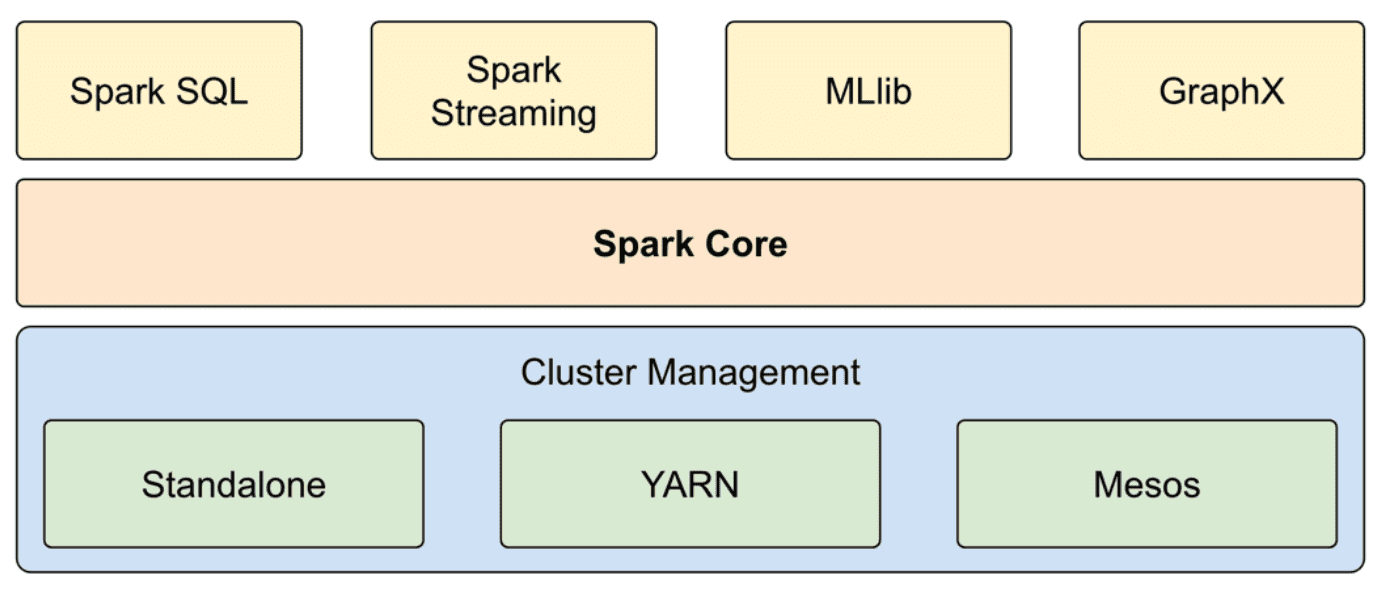
\includegraphics[width=0.8\linewidth]{img/sparkModules.png}
	%TODO https://docs.incorta.com/
	\caption{Archiettura di Spark}
	\label{fig:SparkModules}
\end{figure}
\par Vista la varietà di funzionalità che Spark offre, in questo progetto ci si focalizzerà maggiormente sulle funzionalità di SparkCore e sulle modalità di gestione di Streaming di dati. In entrambi i casi l'analisi verrà svolta si da un punto di vista estereriore di quello che offre il framework che quello interiore, andando a sviscerare le caretteristiche e i punti peculiari (positivi o negativi) che emergono dall'analisi. 
\newline
Si sottolinea che in questo progetto è stata utilizzata l'ultima versione disponibile di Spark, ovvero la \textbf{2.4.4}. Per cui per maggiori dettagli si rimanda al sito di Spark\footnote{\url{https://spark.apache.org/docs/2.4.4/quick-start.html}}.
\subsection{Perchè Spark è così importante?}
L'importanza di Spark è data soprattutto dal fatto che in un'unico framework vengono create interesioni di vario genere che fanno si che esso sia una piattaforma a tutto tondo. Questi punti sintetizzano i motivi principali dell'importanza di Spark:
\begin{itemize}
	\item Astrae la programmazione parallela, non sembra di lavorare su un cluster di computer.
	Nello scenario migliore sembrerà di lavorare con un database (SQL), nel peggiore di lavorare su Collections.
	\item Piattaforma unificata, tutto in un singolo framework.
	\item Facile da usare, leggere e capire.
\end{itemize}
\subsection{Un primo approccio a Spark}
Per prendere confidenzialità con Spark, così come abbiamo fatto con Scala, può essere utile utilizzare la REPL (anche nota come \textbf{spark-shell}). 
Utilizzarla con Spark è molto semplice:
\begin{itemize}
	\item basta andare nell'url \url{https://spark.apache.org/downloads.html} e scaricare l'ultima versione di Spark compresa di Hadoop;
	\item decomprimere la cartella e posizionarsi all'interno di essa da terminale;
	\item a questo punto lanciando il comando \texttt{./bin/spark-shell} partirà la shell.
\end{itemize}
Si può anche memorizzare questo percorso nel path di sistema e accedervi da qualsiasi parte del file system. Aggiungendo a ~/.bashrc:
\begin{itemize}
	\item \texttt{export SPARK\_HOME="percorso della cartella decompressa"} 
	\item \texttt{export PATH=$PATH:$SPARK\_HOME/bin:\$SPARK\_HOME/sbin}
\end{itemize}

Seguendo questo \href{https://bigdata-madesimple.com/learning-scala-spark-basics-using-spark-shell-in-local/}{tutorial} è possibile mettere le mani in pasta in locale su un dataset e esplorare le potenzialità di Spark (in particolare Spark SQL) e, soprattutto, del DLS che esso fornisce.
\section{Internals}
\subsection{Architettura}
É possibile lanciare Spark essenzialmente in \textbf{due modalità}:
\begin{enumerate}
	\item \textbf{interattiva}
	\item \textbf{submit di un job} (in caso di produzione). 
\end{enumerate}
Queste modalità ci aprono al concetto di \textit{master-worker} (PCD) che nel ``dialetto di Spark" è noto come \textbf{``driver-executor"}.
Essenzialmente posso usare Spark con o senza un vero cluster:
\begin{itemize}
	\item \textbf{local mode}: uso in fase esplorativa per iniziare ad usare spark senza un effettivo cluster.
	\item \textbf{con cluster}
	\begin{itemize}
		\item \textbf{client mode}: il driver è nel client, per cui è preferibile usarla in fase di debug;
		\item \textbf{cluster mode}: il driver è nel cluster, la uso in produzione.
	\end{itemize}
\end{itemize}
Quando eseguo Spark lo stato dei processi è visibile in una pagina web che viene linkata nel esecuzione del progesso (la \textbf{Spark UI}), in essa è possibile visualizzare come viene effettivamente distribuito il lavoro, lo stato del lavoro e i DAG. %TODO

\textit{Chi controlla il cluster? Come Spark ottiene le risorse per driver e executor?}
Il \textit{cluster manager}, il quale non viene offerto da Apache Spark. Tra i più noti abbiamo:
\begin{itemize}
	\item\textbf{Apache YARN} per Hadoop;
	\item\textbf{Apache Mesos} (general purpose);
	\item\textbf{Kubernetes}: Google, non ancora adatto per fasi di produzione
	\item\textbf{StandAlone} facile e veloce, non ancora adatto per fasi di produzione. %TODO check
\end{itemize}


\subsection{RDDs  e tasks}
\subsubsection{Resilient Distributed Datasets (RDDs)}
Spark ruota attorno al concetto di RDD, ovvero una collection fault-tollerant che può essere processata in parallelo. Ci sono due modi per creare un RDD: parellelizzando una collezione esistente nel tuo driver program o facendo riferimento a un archivio di dati esterno (come filesystem condivisi, HDFS, Hbase o qualsiasi input che ha dati in formato Hadoop).

\subsubsection{RDDs e conseguenze}
Poichè Dataset e DataFrame (API di dati strutturati) ereditano da RDDs (non strutturati), capendo questi ultimi possiamo capire come effettivamente viene distribuito il lavoro tra gli executors.

Quando viene letto un file è possibile specificare il numero di \textbf{partizioni di un RDD} che (guarda caso) coincide con il corrispondente \textbf{numero di task}.
Ovviamente, numero executors e di task sono effettivamente correlati e quindi bisogna specificare il numero di conseguenza.

Si lavora in \textbf{stage}, uno stage rappresenta un periodo (una o più funzione chiamata sui dati) in cui non è necessario uno shuffle, ovvero non è necessario spostare i dati tra le partizioni. Se i dati devono muoversi (es. reduceByKey) bisogna ripartizionare i dati (\textit{shuffle \& sort}).
Con `collect` si ritorna dagli executor al driver.

%TODO Nota interessante, in Scala, DataFrame è così definito ``type DataFrame = Dataset[Row]" \footnote{\url{https://spark.apache.org/docs/2.4.4/api/scala/index.html}}, ciò significa che su un DataFrame posso chiamare tutti i metodi del Dataset.

\subsection{Execution Model} %TODO
\begin{itemize}
	\item Crea DAG di RDDs per rappresentare la computazione;
	\item Crea piano di esecuzione logico del DAG;
	\item pipeline il più possibile %TODO
	\item divide in \textbf{stages}
	\item Schedula e esegue i tasks:
	\item divide ogni stage in task
	\item task = dati + computazione
	\item esegue tutti i task di uno stage prima di andare avanti
\end{itemize}

\subsection{Di più sullo shuffle}
Note importanti sullo shuffle sono:
\begin{enumerate}
	\item è pull based e non push based;
	\item scrive file intermedi nei dischi
\end{enumerate}
Bisognate tenere d'occhio il \textbf{numero di partizioni} perchè possono fondamentalmente esserci due situazioni.
\begin{enumerate}
	\item numero troppo \textbf{basso}:
	\begin{itemize}
		\item poca concorrenza
		\item più suscettibile a \textit{``data skew"} (spostamento di dati)
		\item maggiore uso della memoria in operazioni che richiedono Shuffle (groupBy, sortByKey, reduceByKey, etc.)
	\end{itemize}
	\item numero troppo \textbf{alto}: problemi opposti, dati troppo sparsi e non viene sfruttato il partizionamento.
\end{enumerate}
Un numero appropiato di solito è tra 100 e 10000.
Bisogna fissare questo numero nell'intervallo compreso tra:
\begin{itemize}
	\item \textbf{lower bound}:  almeno circa il doppio del numero di core di un cluster;
	\item \textbf{upper bound}: essere sicuri che un task venga eseguito in almeno 100ms.
\end{itemize}

%TODO (da vedere https://databricks.com/session/a-deeper-understanding-of-spark-internals da min. 22)

\section{Moduli di Spark}
\subsection{Iniziare a lavorarare con Spark e gli RDDs}
Per iniziare a usare Spark bisogna comprendere due concetti principali che sono lo \textit{SparkContext} e la \textit{SparkSession}. %TODO
Per ciascuna JVM ci può essere al più una \textit{SparkContext}.

\par Ci sono due operazioni fondamentali che vengono fatte sui dati, che rispecchiano essenzialemente il principio \textit{map-reduce}:
\begin{itemize}
	\item \textbf{transformations}: ovvero operazioni di map \textit{map}, sono lazy l'eventuale azione su di essa applicherà la trasformazione. Eventualmente è possibile rendere questi cambiamenti persistenti (con l'opportuno persist), altrimenti non lo sono.
	\item \textbf{actions}: ovvero operazioni di map \textit{reduce}.
\end{itemize}
La Figura \ref{fig:RDDs} mostra l'intero meccanismo di RDDs e trasformazioni e azioni.
\begin{figure}
	\centering 
	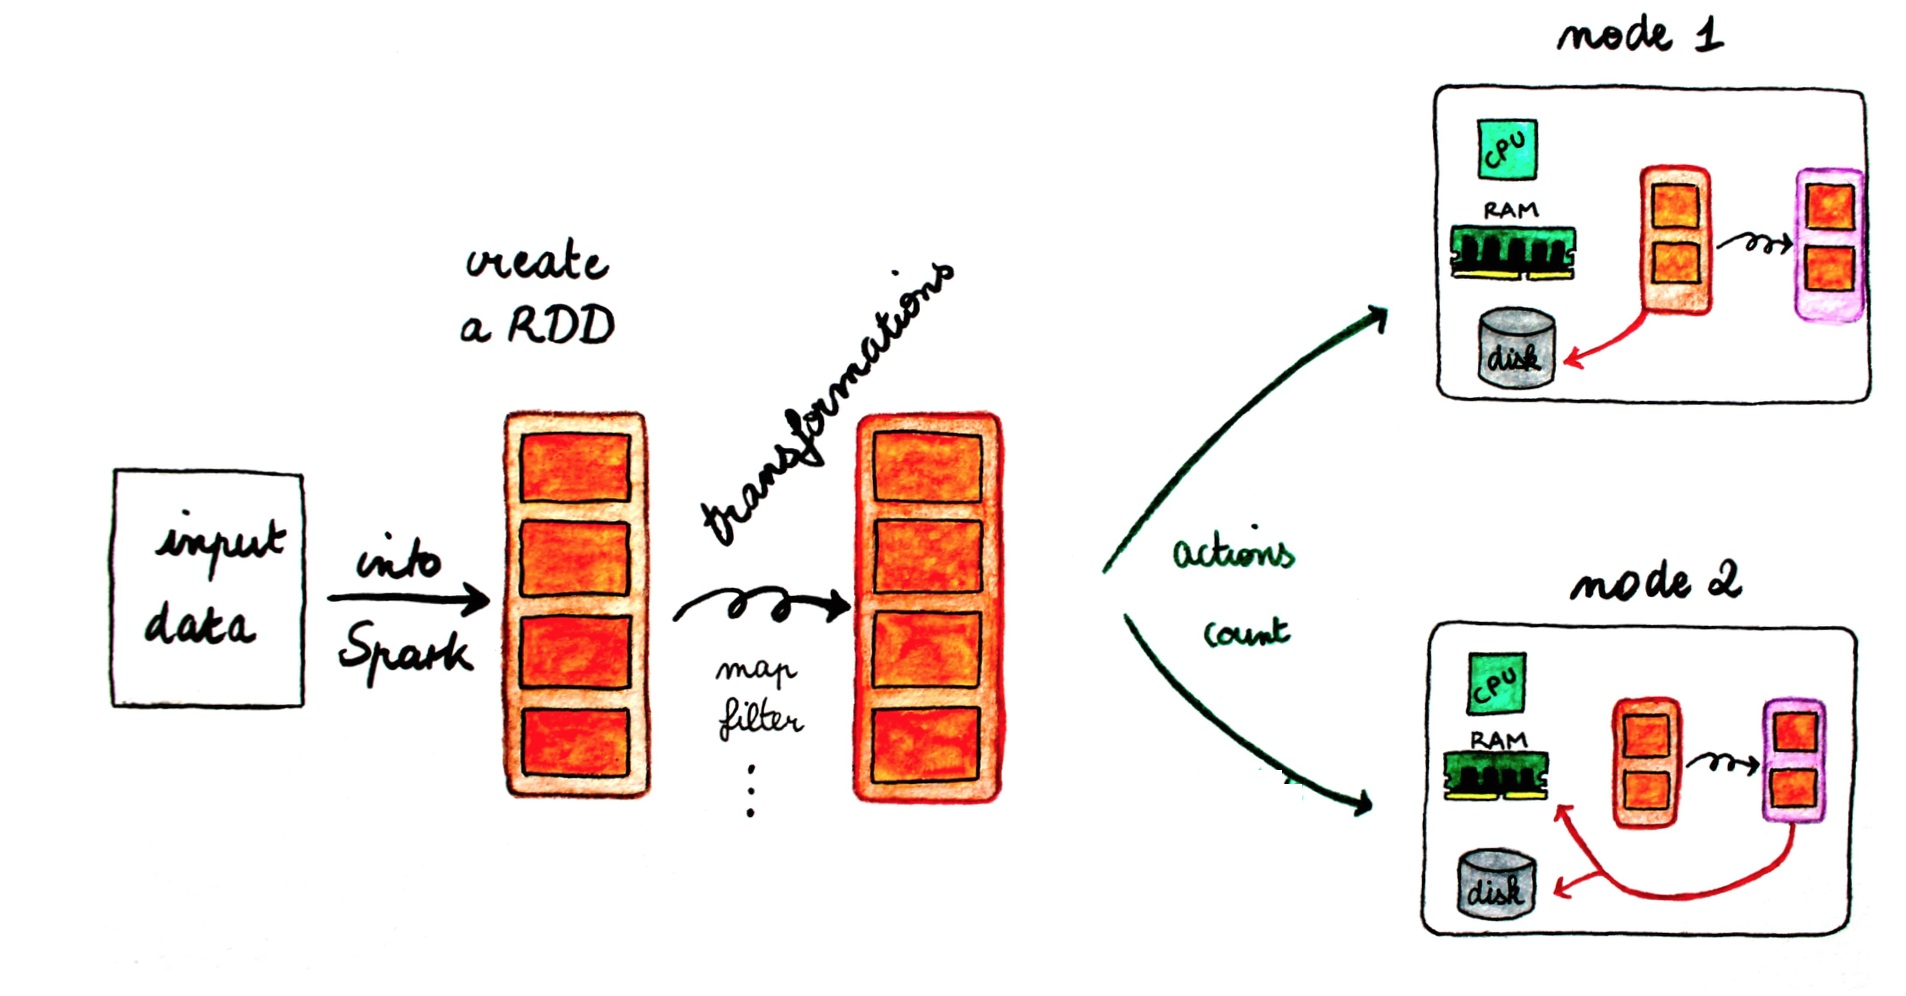
\includegraphics[width=1\linewidth]{img/rdds.png}
	\caption{RDDs e meccanismo di trasformations e actions.}
	%TODO Immagine tratta da \citeweb{http://sparkforbeginners.blogspot.com}
	\label{fig:RDDs}
\end{figure}
\par Per passare funzioni a Spark nel sito viene mostrato come sfruttare map su un RDDs applicandoci una propria funzione che prende in input un dato dello stresso tipo di quello contenuto nel RDDs. Secondo me questo aspetto da un lato obbliga il programmatore ad appoggiarsi alle API fornite dal framework e quindi ottimizzate da Spark, dall'altro pone dei limiti nel come il programmatore vuole approcciarsi ai dati. Limite che viene abbastanza ridotto dalla potenza e dalla facilità di comprensione del DLS che Spark mette a disposizione.
\par Per quanto riguarda il \textbf{caching}, oltre a persistent, esistono modalità per specificare a quale memoria far riferimento e funziona anche su dati presenti in molti nodi.
\par Se andassi ad applicare \texttt{collect()} su una grande quantità di dati potrei incorrere in un \textit{``out of memory"}, per cui bisogna applicare concetti simili a quelli visti durante il corso di PPS. Ad esempio anzichè fare una stampa di tutti i dati, si vanno recuperare i primi N record con una \texttt{take(N)}.
\subsection{Machine Learning Library (MLlib)}
Questo modulo consiste in:
\begin{itemize}
	\item \textit{Algoritmi di Machine Learning}: come classificazione, regressione, clustering e filtering collaborativo.
	\item \textit{Featurization}: estrazione delle feature, transformazione, riduzione della dimensionalità e selezione.
	\item \textit{Pipelines}: tool per costruire, valutare e fare tuning di pipeline di ML.
	\item \textit{Persistenza}: salvare e eseguire algoritmi, modelli e pipeline.
	\item \textit{Utility}: algebra lineare, statistica, gestione dati, etc.
\end{itemize}
\subsection{Spark SQL}
Supporto a dati strutturati, fornisce maggiori ottimizzazioni rispetto a RDD. L'interazione con i dati è possibile in vari modi, tra cui SQL e Dataset API.
Nella computazione viene usato un unico engine di esecuzione, il programmatore può esprire le cose nel modo che ritiene più naturale. Uso di Hive, JDBC, etc. 
Non credo questo sia interessante sul lato PPS. %TODO
\subsubsection{Dataset API}
Operazioni con cui interrogare il Dataset. 
Un Dataset si può creare anche `on the fly" da un file di testo o appartenere a determinati formati (es. Hadoop HDFS) o trasformando altri Dataset.
Nelle interrogazioni che lo richiedono vengono passate funzioni, per cui possono entrare in gioco aspetti di PPS. Questa parte verrà meglio sviscerata in seguito. %TODOs
\subsection{GraphX Programming}
Componente Spark per Grafi e calcolo graph-parallel.

Ad alto livello viene estratto il concetto di RDD introducendo l'estensione Graph, in Figura \ref{fig:GraphX} viene mostrata la costruzione del grafo a partire dai dati grezzi.
Ci sono varie operazioni a supporto di questo concetto, anche algoritmi e builder per l'analisi.
\begin{figure}[H]
	\centering 
	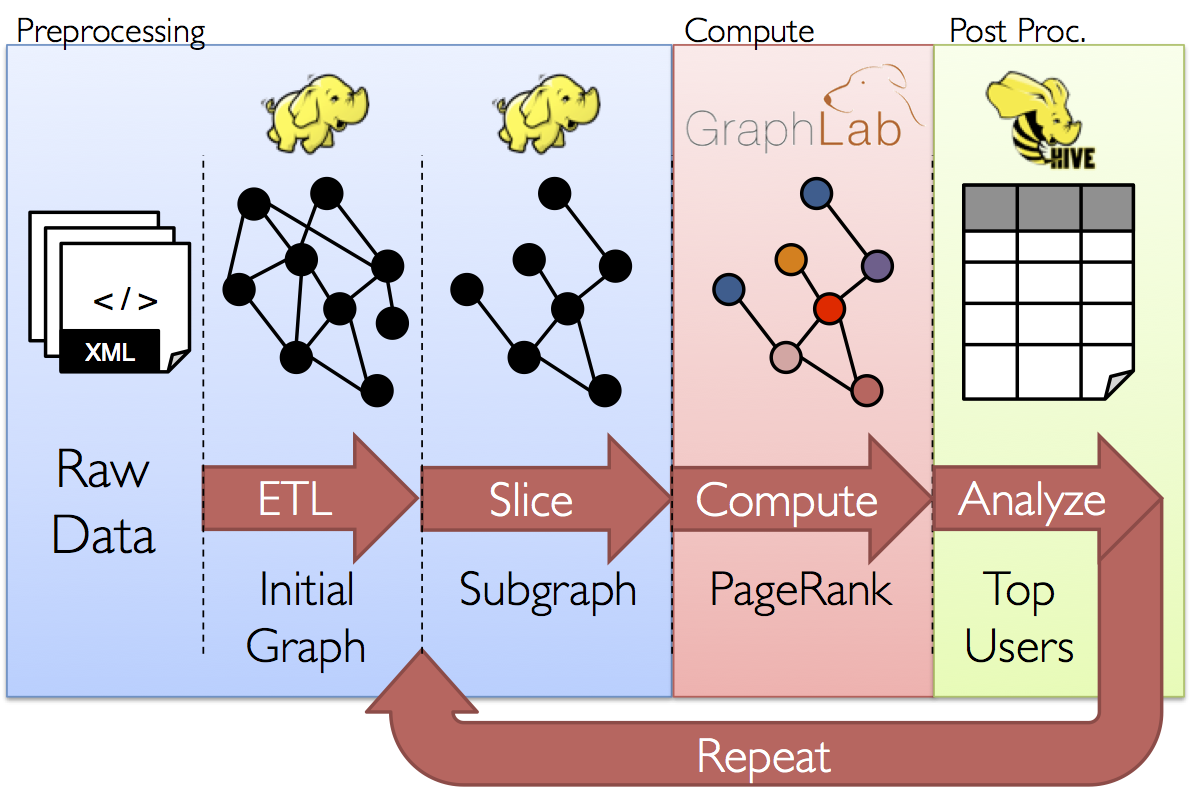
\includegraphics[width=0.8\linewidth]{img/graph_analytics_pipeline.png}
	\caption{Funzionamento di GraphX.}
	%TODO Immagine tratta da \citeweb{http://https://spark.apache.org/}
	\label{fig:GraphX}
\end{figure}
Quindi userei questa estensione quando nella natura dei dati ci sono legami che vengono meglio rappresentati da un grafo,
prima di dare in pasto i dati a GraphX potrebbero servire minime operazioni per renderli "compatibili" con la visione a grafo.
Nella costruzione vengono richiesti:
\begin{itemize}
	\item RDD dei vertici;
	\item RDD degli edge;
	\item un vertice di default (pozzo).
\end{itemize}
\subsection{SparkR (R on Spark)}
SparkR è un pacchetto R che fornisce un frontend leggero per utilizzare Apache Spark da R. In Spark 2.4.4, SparkR fornisce un'implementazione di data frame distribuiti che supporta operazioni come selezione, filtro, aggregazione ecc. (simile a data frame R, dplyr) ma su set di dati di grandi dimensioni. SparkR supporta inoltre l'apprendimento automatico distribuito tramite MLlib.

\subsection{Moduli per lavorare con stream di dati}
\subsubsection{Spark Streaming}
\subsubsection{Spark Structured Streaming}
\begin{figure}[H]
	\centering 
	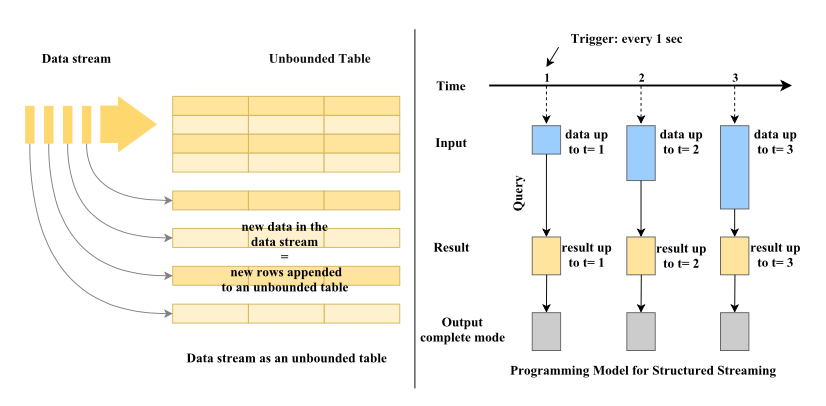
\includegraphics[width=0.8\linewidth]{img/sparkStructuredStreaming.png}
	\caption{Come Spark Structured Streaming mantiene i dati.}
	%TODO Immagine tratta da \citeweb{https://link.springer.com/chapter/10.1007/978-1-4842-4961-1\_3}
	\label{fig:StructuredStreaming}
\end{figure}

\end{document}
    
    
